\section{چارچوب الگوریتم چند هدفه \lr{REMARK}}
به‌منظور اجراي فرآيند بهينه‌سازی چند هدفه توسط \lr{REMARK}، دو ايده در اين بخش ادغام شده است. اين دو ايده تا حد بسيار زيادی مشابه بهينه‌سازي چندهدفه در الگوريتم \lr{PSO} است. در ايده اول، هدف ذخیره پاسخ‌های بهينه پارتو نقاط غالب است. ايده دوم نيز استراتژی اشتراک گذاشتن بهترین تجربه هر متضاضی با دوستان خود است. مدل عرضه و تقاضا در تک هدفه و چند هدفه یکسان است، در بخش‌های
\ref{sec:market_model_multi}
و 
\ref{sec:intraction_multi}
به تغیرات الگوریتم جهت بهینه‌سازی چند هدفه اشاره شده است.



%\lr{
%\begin{algorithm}[H]
%	\KwData{this text}
%	\KwResult{how to write algorithm with \LaTeX2e }
%	initialization\;
%	\While{not at end of this document}{
%		read current\;
%		\eIf{understand}{
%			go to next section\;
%			current section becomes this one\;
%		}{
%			go back to the beginning of current section\;
%		}
%	}
%	\caption{How to write algorithms}
%\end{algorithm}
%}
\subsection{مدل بازار}\label{sec:market_model_multi}

مدل بازار در بخش
\ref{sec:market_model}
به طور کامل بررسی شد. مدل بازار در بهینه‌سازی چند هدفه بسیار شبیه به تک هدفه است. در چند هدفه برای بازار مستغلات یه مفهوم دیگر به نام محله مستغلات در نظر گرفته شده است. در این مفهوم به طور معمول عرضه‌کننده و تقاضا کننده به ندرت از محله خود خارج می‌شوند اما به جهت جست‌و‌جو بهتر الگوریتم این امکان به صورت تصادفی گذاشته شده است.

\subsection{تعامل بازیگران و اصول کار الگوریتم چند هدفه}\label{sec:intraction_multi}
 در بخش \ref{sec:intraction}
به‌طور کامل به تعامل بین افراد پرداخته است و در این بخش از تکرار جزییات آن خودداری شده است و صرفا کلیت موضوع و تفاوت‌ها بررسی شده است.
 تقاضا‌کنندگان برای مهاجرت به صورت تصادفی دوست پیدا می‌کنند و از تجربیات آن‌ها استفاده می‌کنند. در چند حالته فرض شده است هر تقاضاکننده سعی دارد در محله قبلی خود بماند. فرایند انتخاب کردن محله به صورت است که متقاضی با دوستان خود ارتباط بر قرار می‌کند و بعد از آنکه داده‌های دوست‌های خود را گرفت پارتو بهینه آن را بدست می‌آورد. لیست بدست آمده کاندیدهای جدید برای مهاجرت هستند. در این لیست هیچ یک از کاندیدها بر کاندید دیگری مسلط نیست. برای انتخاب ملک جدید جهت مهاجرت متقاضی سعی دارد در محله خود بماند پس هر چه فاصله‌ کاندید‌‌ه‌ها از او کمتر باشد مناسب‌تر است. در نهایت متقاضی برای مهاجرت از یک پدیده تصافی جهت انتخاب ملک جدید استفاده می‌کند، به این صورت که، هر چه ملک جدید نزدیک‌تر باشد، شانس انتخاب آن نیز بیشتر است. این امر باعث می‌شود هر متقاضی در یک محله جست‌وجو کند (استخراج به خوبی انجام شود) و یک ناحیه از پارتو را بررسی کند از طرفی به دلیل اینکه، از فرایند تصادفی جهت مهاجرت استفاده می‌کند و انتخاب دوست نیز تصادفی است و تابعی از فاصله نیست، سبب می شود که جست‌و‌جو زیاد شود و احتمال پیدا کردن جواب بهتر را بالا رود.
 
 برای عرضه‌کننده هم روش بالا که برای تقاضاکننده بیان شد استفاده شده است. به این صورت که عرضه‌کننده سعی دارد در یک محله عرضه کند و برای ساخت و ساز نیز به صورت تصادفی اشاره شده عمل می‌کند.
 
 
 روش اشاره شده سعی دارد که تعدادی متقاضی و عرضه‌کننده را در یک ناحیه پارتو نگهدارد، که از تعامل این دو نوع بازیگر جست‌وجو و استخراج برای آن ناحیه از پارتو انجام شود و در نهایت با استفاده از کل بازیگران، مجموعه‌ی کامل‌تر و بهینه‌تری از پارتو بهینه بدست آورد.
 
 \section{پیاده‌سازی}
 در این قسمت به پیاده‌سازی الگوریتم بهینه‌سازی چند هدفه پرداخته شده است. کد این الگوریتم در زبان پایتون\LTRfootnote{Python 3}
 نوشته شده است و کتابخانه‌های استفاده شده جهت نصب نیز آورده شده است. در پیاده‌سازی از تابع‌های هدف هم و جهت‌ غیر هم جهت استفاده شده است تا عملکرد الگوریتم بهتر دیده شود.
 برای تصویر سازی بهتر نتایج بهینه‌سازی در دو و سه بعد به صورت نمودار آورده شده است. این کار صرفا سبب دید بهتر مجموعه بهینه پارتو می‌شود و الگوریتم پیاده‌سازی شده قابلیت پیاده‌سازی در تمامی ایعاد را دارد.
 
\subsection{پیاده‌سازی توابع هم جهت}
 توابع هدف هم جهت و به صورت زیر تعریف شده‌اند.
 \lr{
\begin{equation}
	\boldsymbol{f} = 
	\begin{cases}
		\sum_{i=0}^{D}z_j^2 \\
		\left(\sum_{i=1}^{D}\left(\sum_{j=1}^{i}z_j\right)^2\right)(1+0.4\left\|N(0, 1))\right\|) 
	\end{cases}
\end{equation}
}

\begin{figure}[H]
	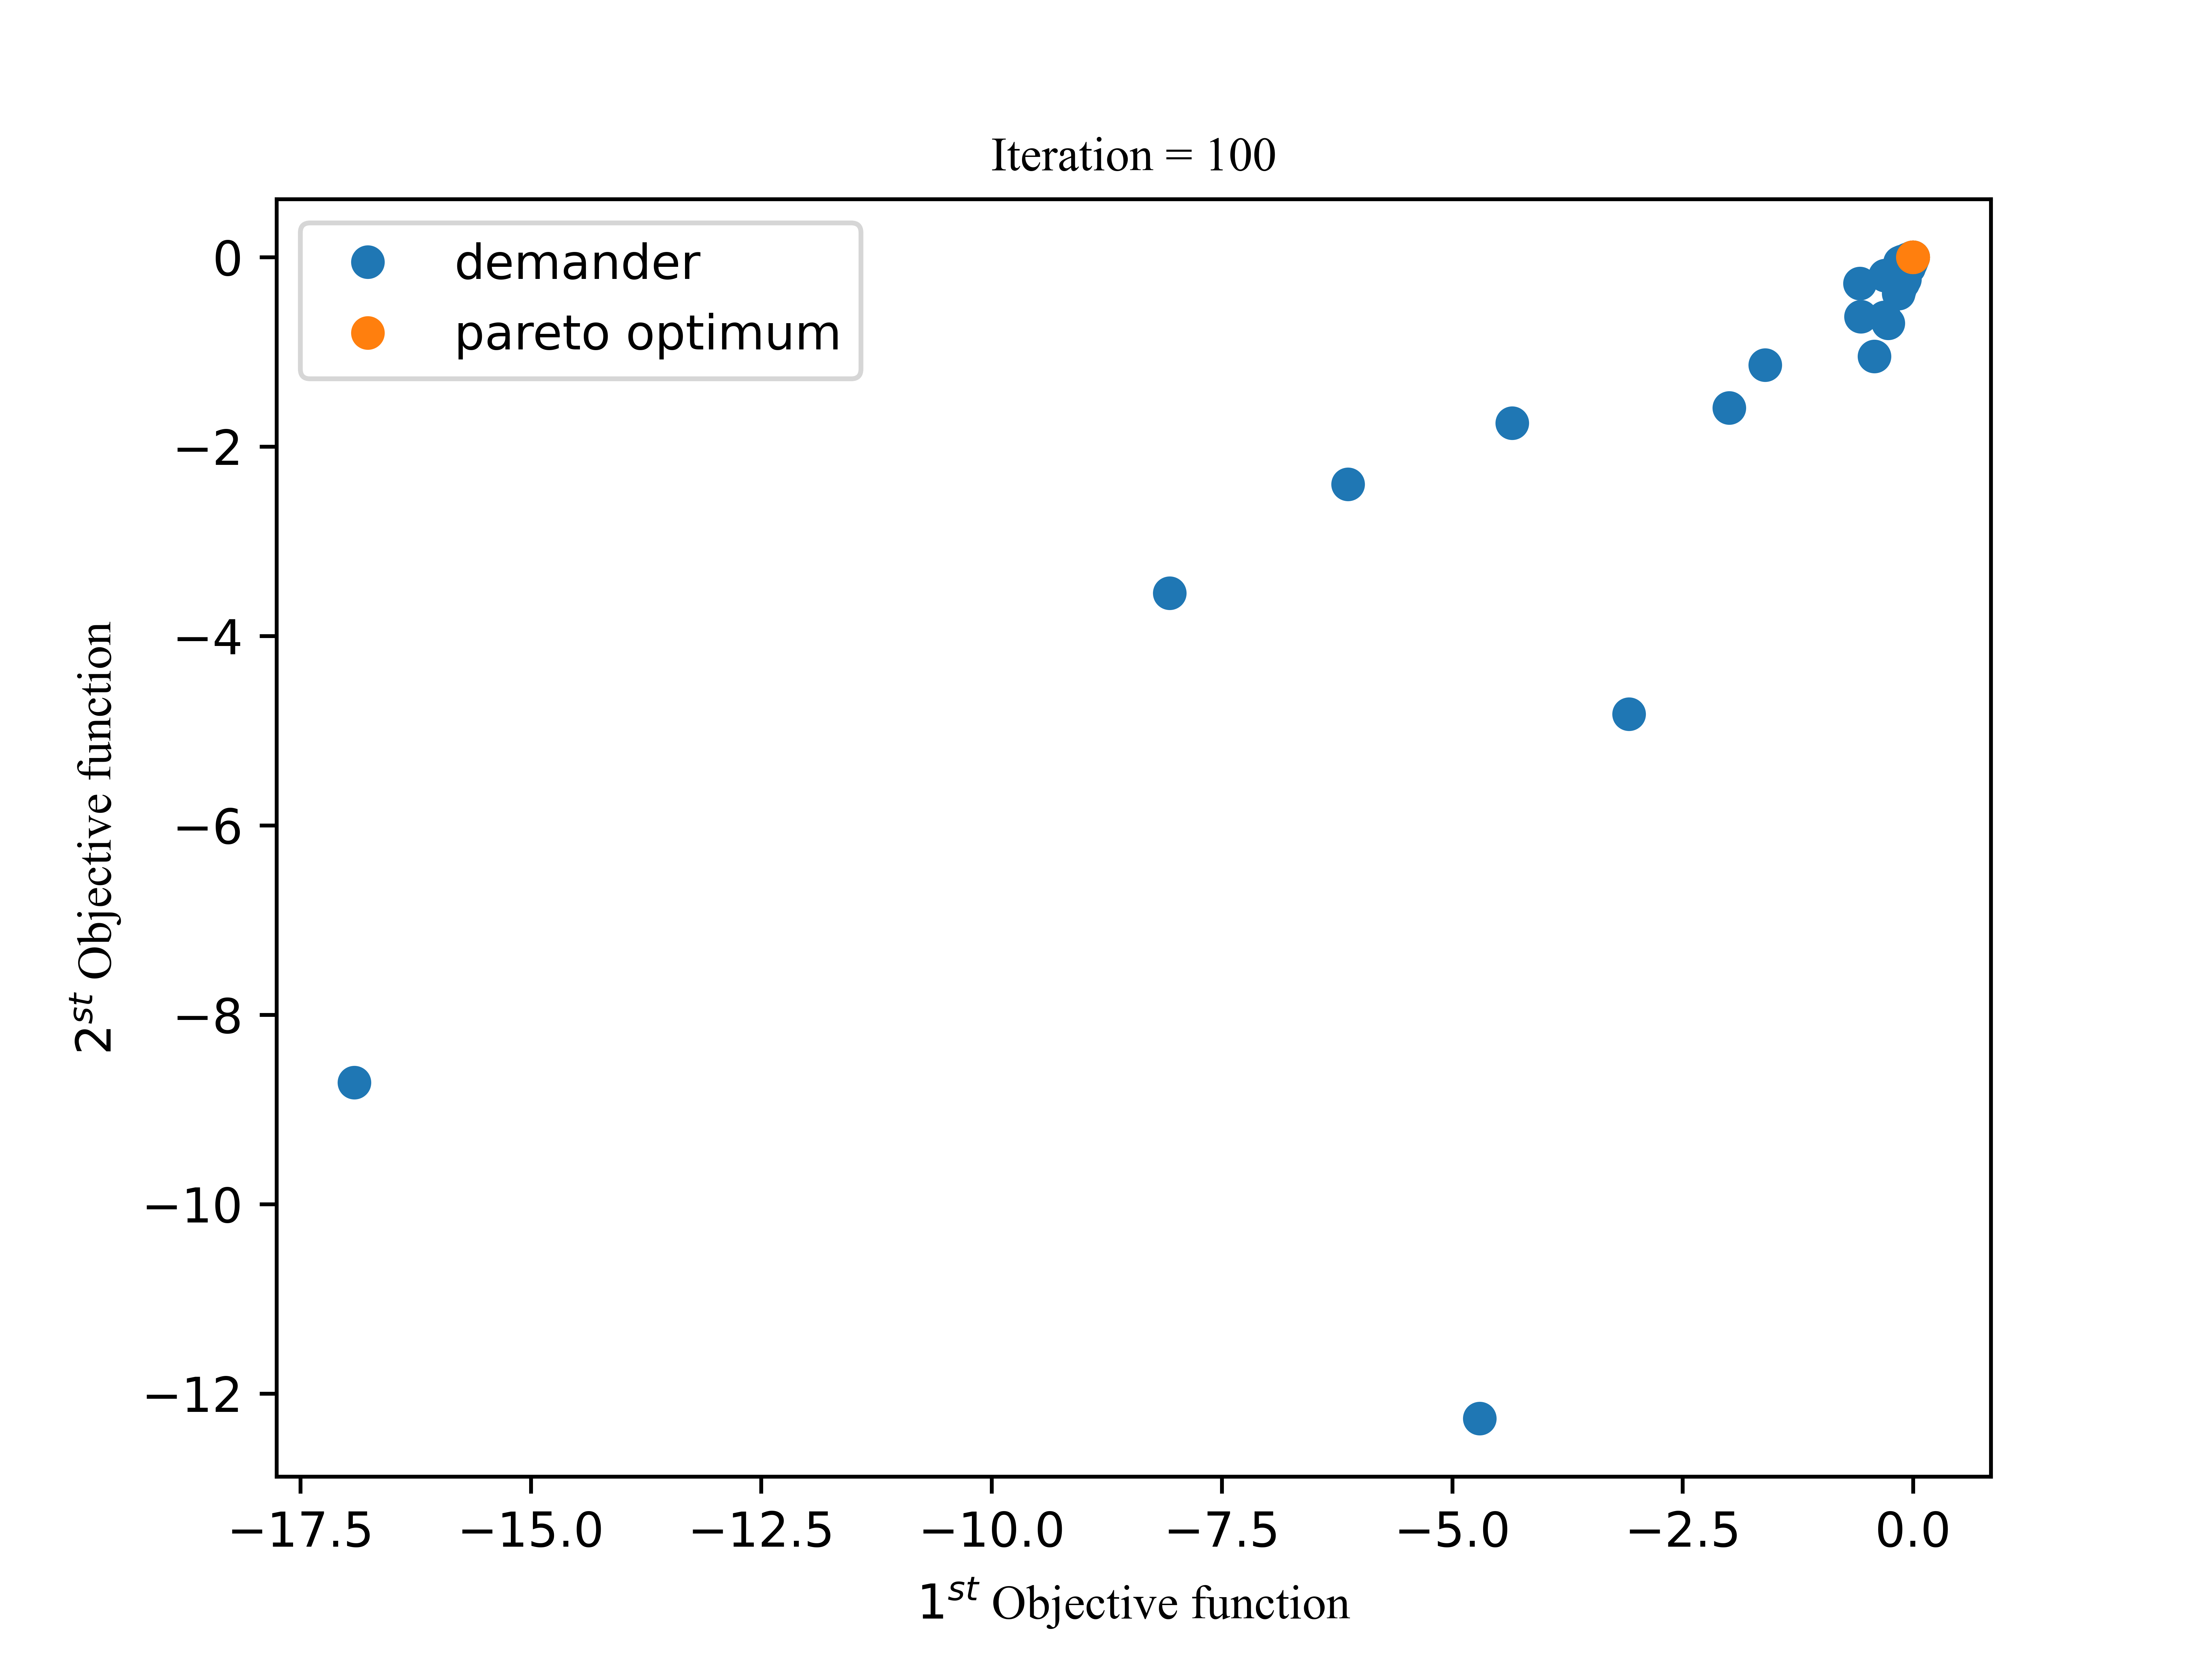
\includegraphics[width=16cm]{../Figure/results/cooperative_2d.png}
	\centering
	\caption{مکان تقاضا‌کنندگان و بهینه پارتو در بهینه‌سازی چند هدفه هم جهت دو بعدی}
\end{figure}

\begin{table}[H]
		\caption{پارامترهای بهینه‌سازی چند هدفه هم جهت دو بعدی}
		\centering
		\begin{tabular}{|c|c|c|}
			\hline
			مقدار & پارامتر\\
			\hline
		$	80$ 
		& تعداد تقاضا‌کنندگان\\
			$4$ 
			& نسبت تقاضاکنندگان به عرضه‌کنندگان \\
	 	$	4 $
	 	& نسبت تقاضاکنندگان به تعداد گروه دوستان\\
	 	$20$ 
	 	& نسبت زمان ساخت به زمان هر تکرار \\
	 		$0.7 $ &$K_{\sigma_D}$ \\
	 		$0.7$ &$K_{\sigma_S}$ \\
	 		$0.4$ &$K_{n_S}$ \\
	 		
			\hline
		\end{tabular}
\end{table}

\begin{equation}
	\boldsymbol{f} = 
	\begin{cases}
		\sum_{i=0}^{D}z_j^2 \\
		\left(\sum_{i=1}^{D}\left(\sum_{j=1}^{i}z_j\right)^2\right) \\
		\left(\sum_{i=1}^{D}\left(\sum_{j=1}^{i}z_j\right)^2\right)(1+0.4\left\|N(0, 1))\right\|) 
	\end{cases}
\end{equation}

\begin{figure}[H]
	\centering
	\subfloat[]{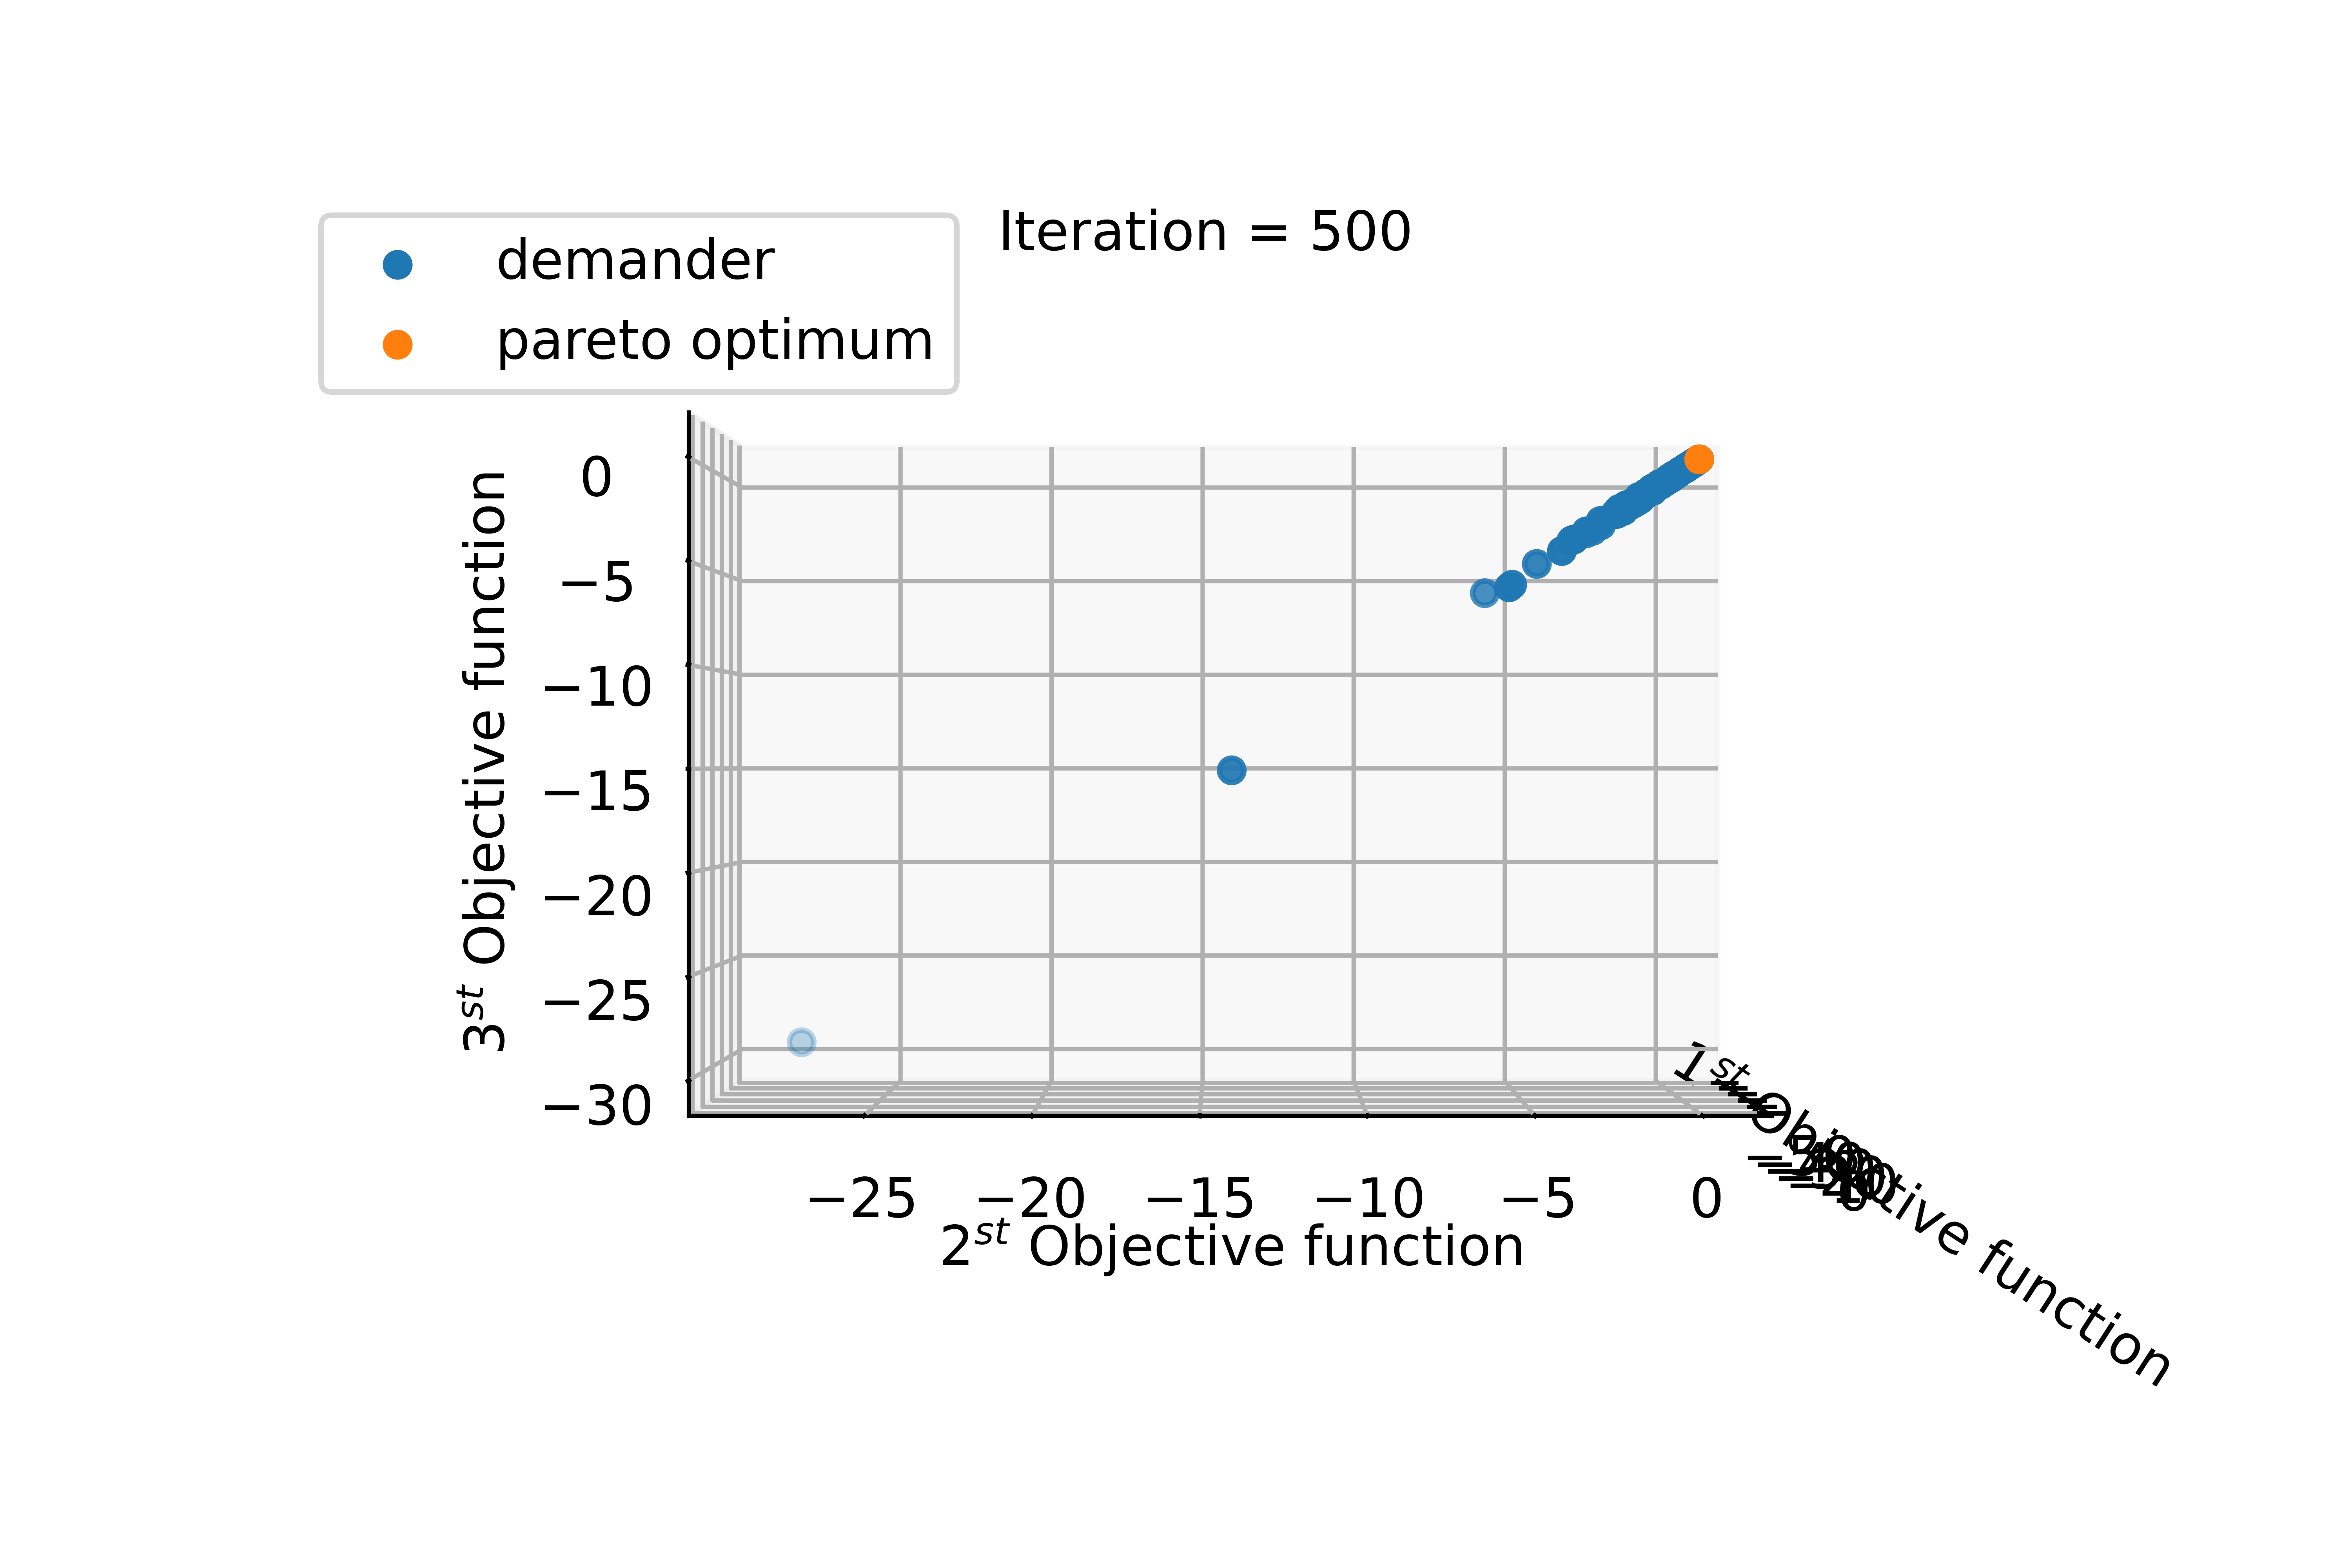
\includegraphics[width=.5\linewidth]{../Figure/results/cooperative_3d_1.png}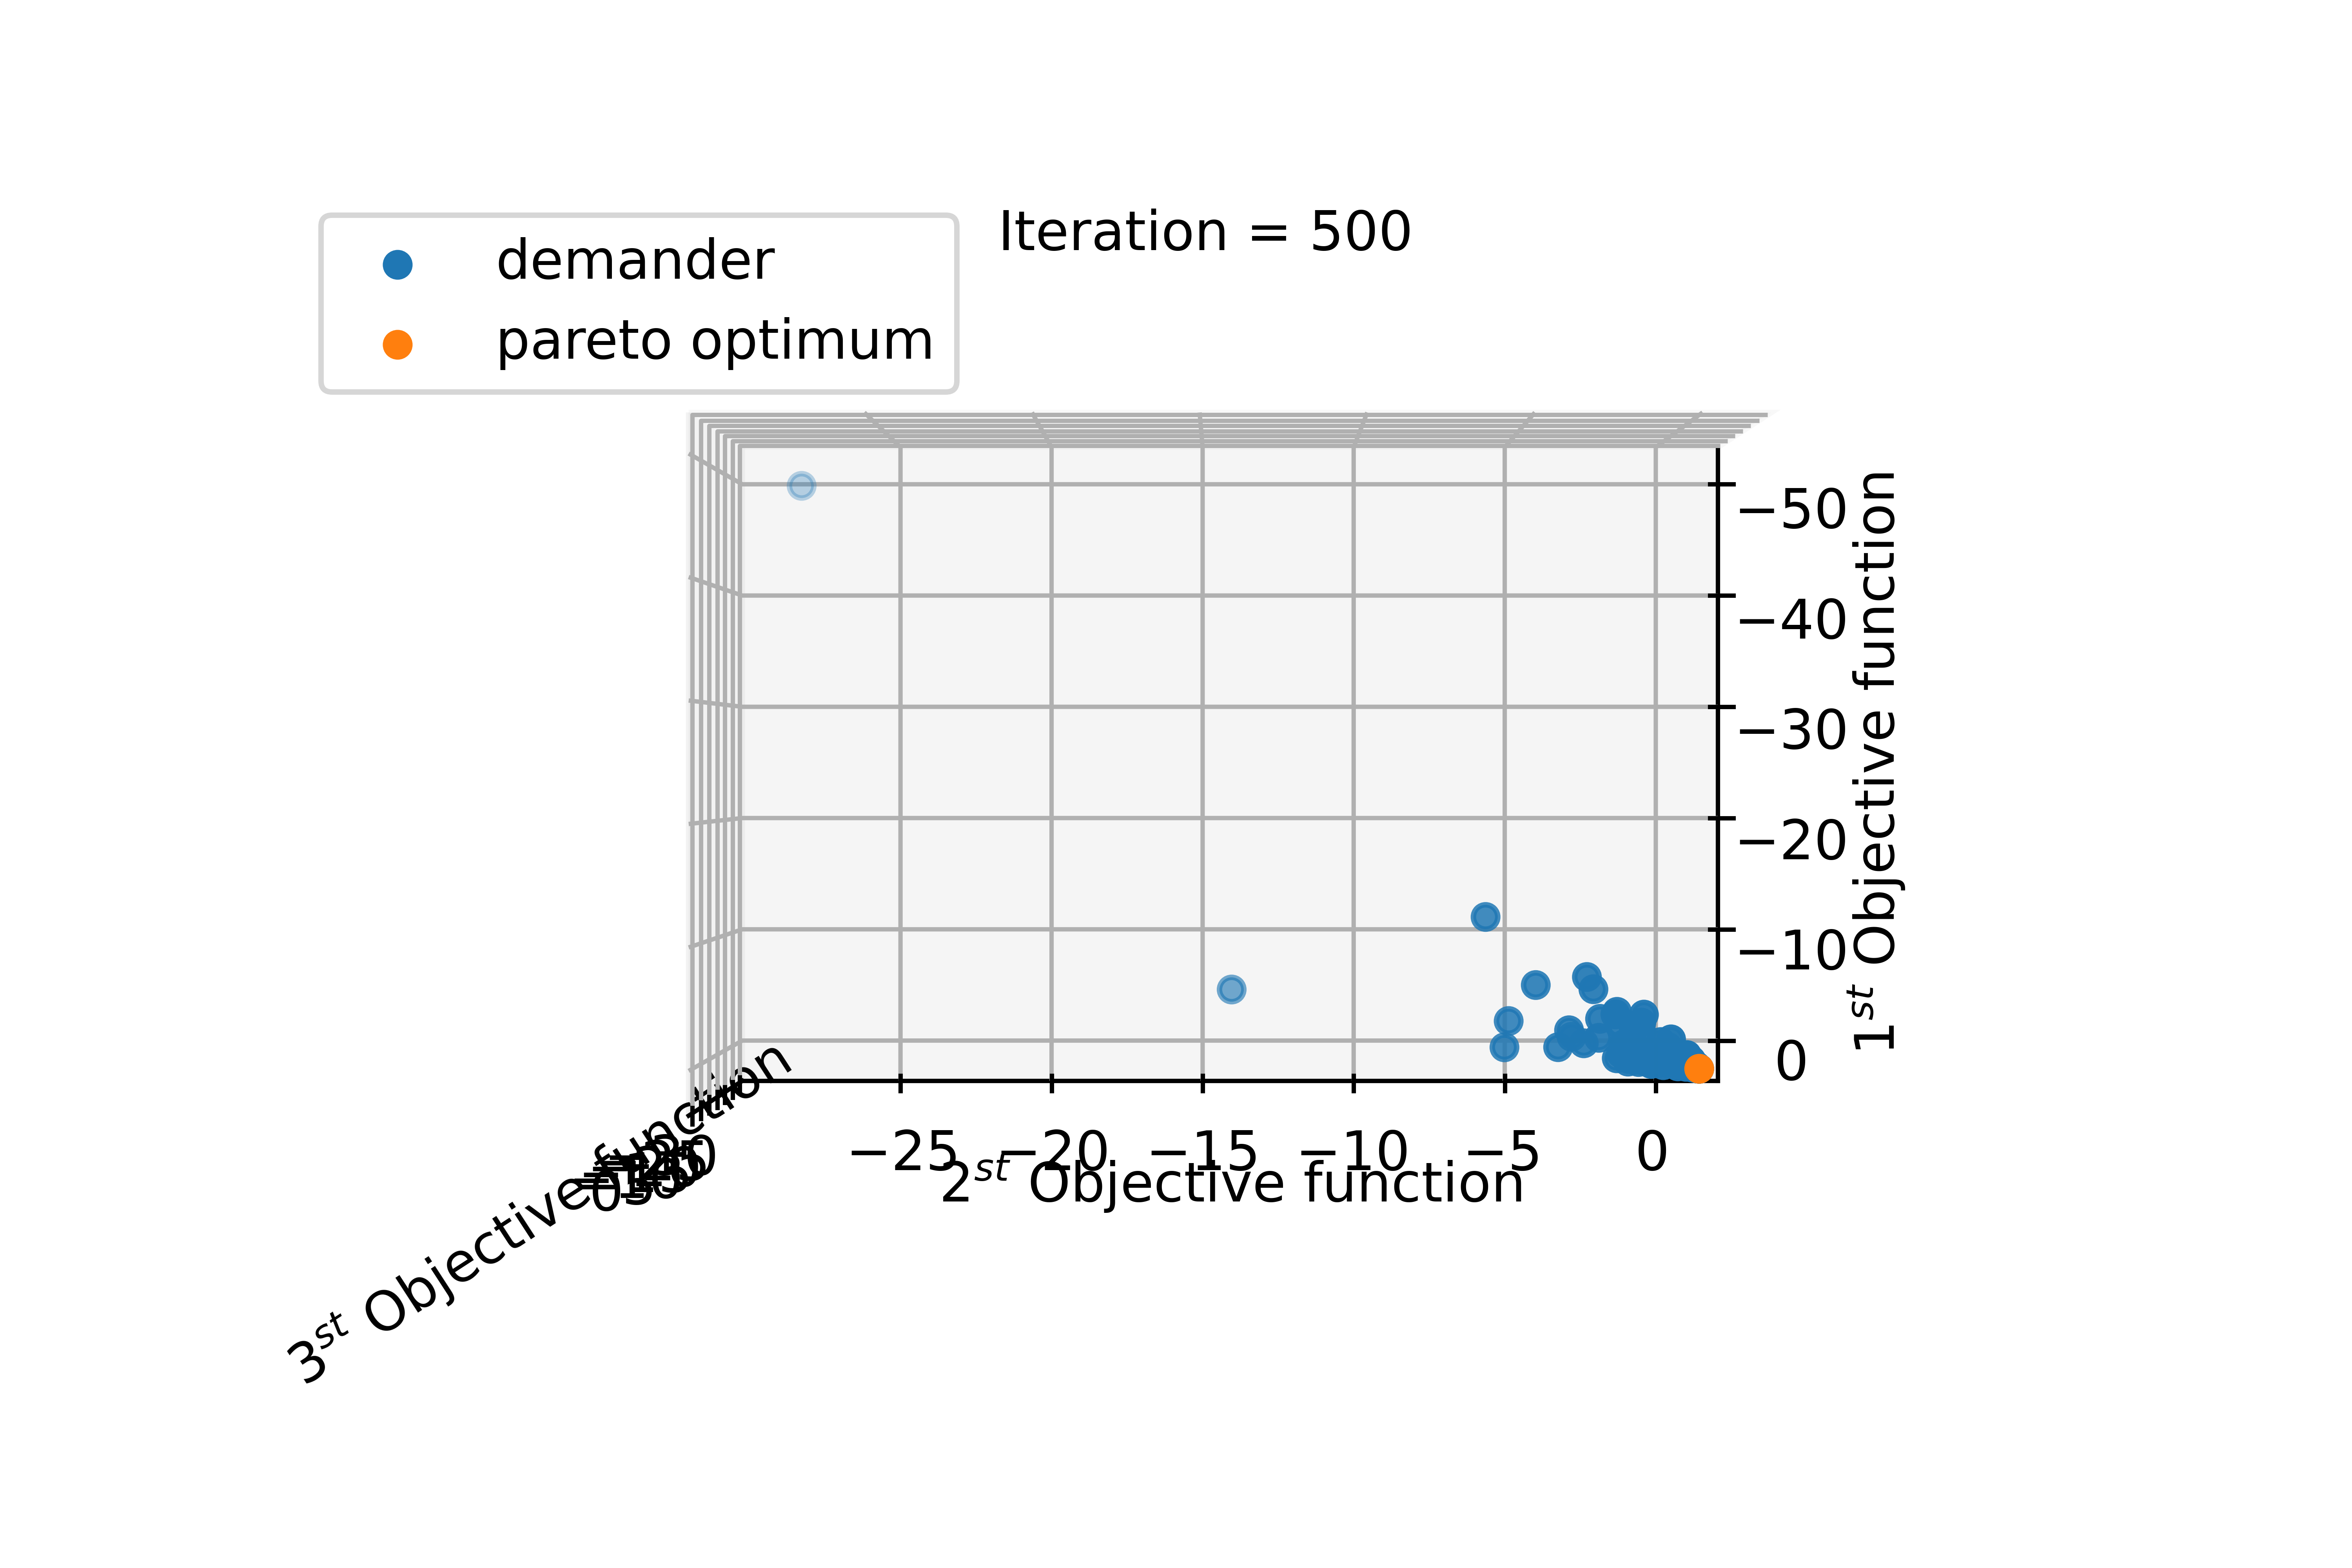
\includegraphics[width=.5\linewidth]{../Figure/results/cooperative_3d_2.png}}
	\hfill
	\subfloat[]{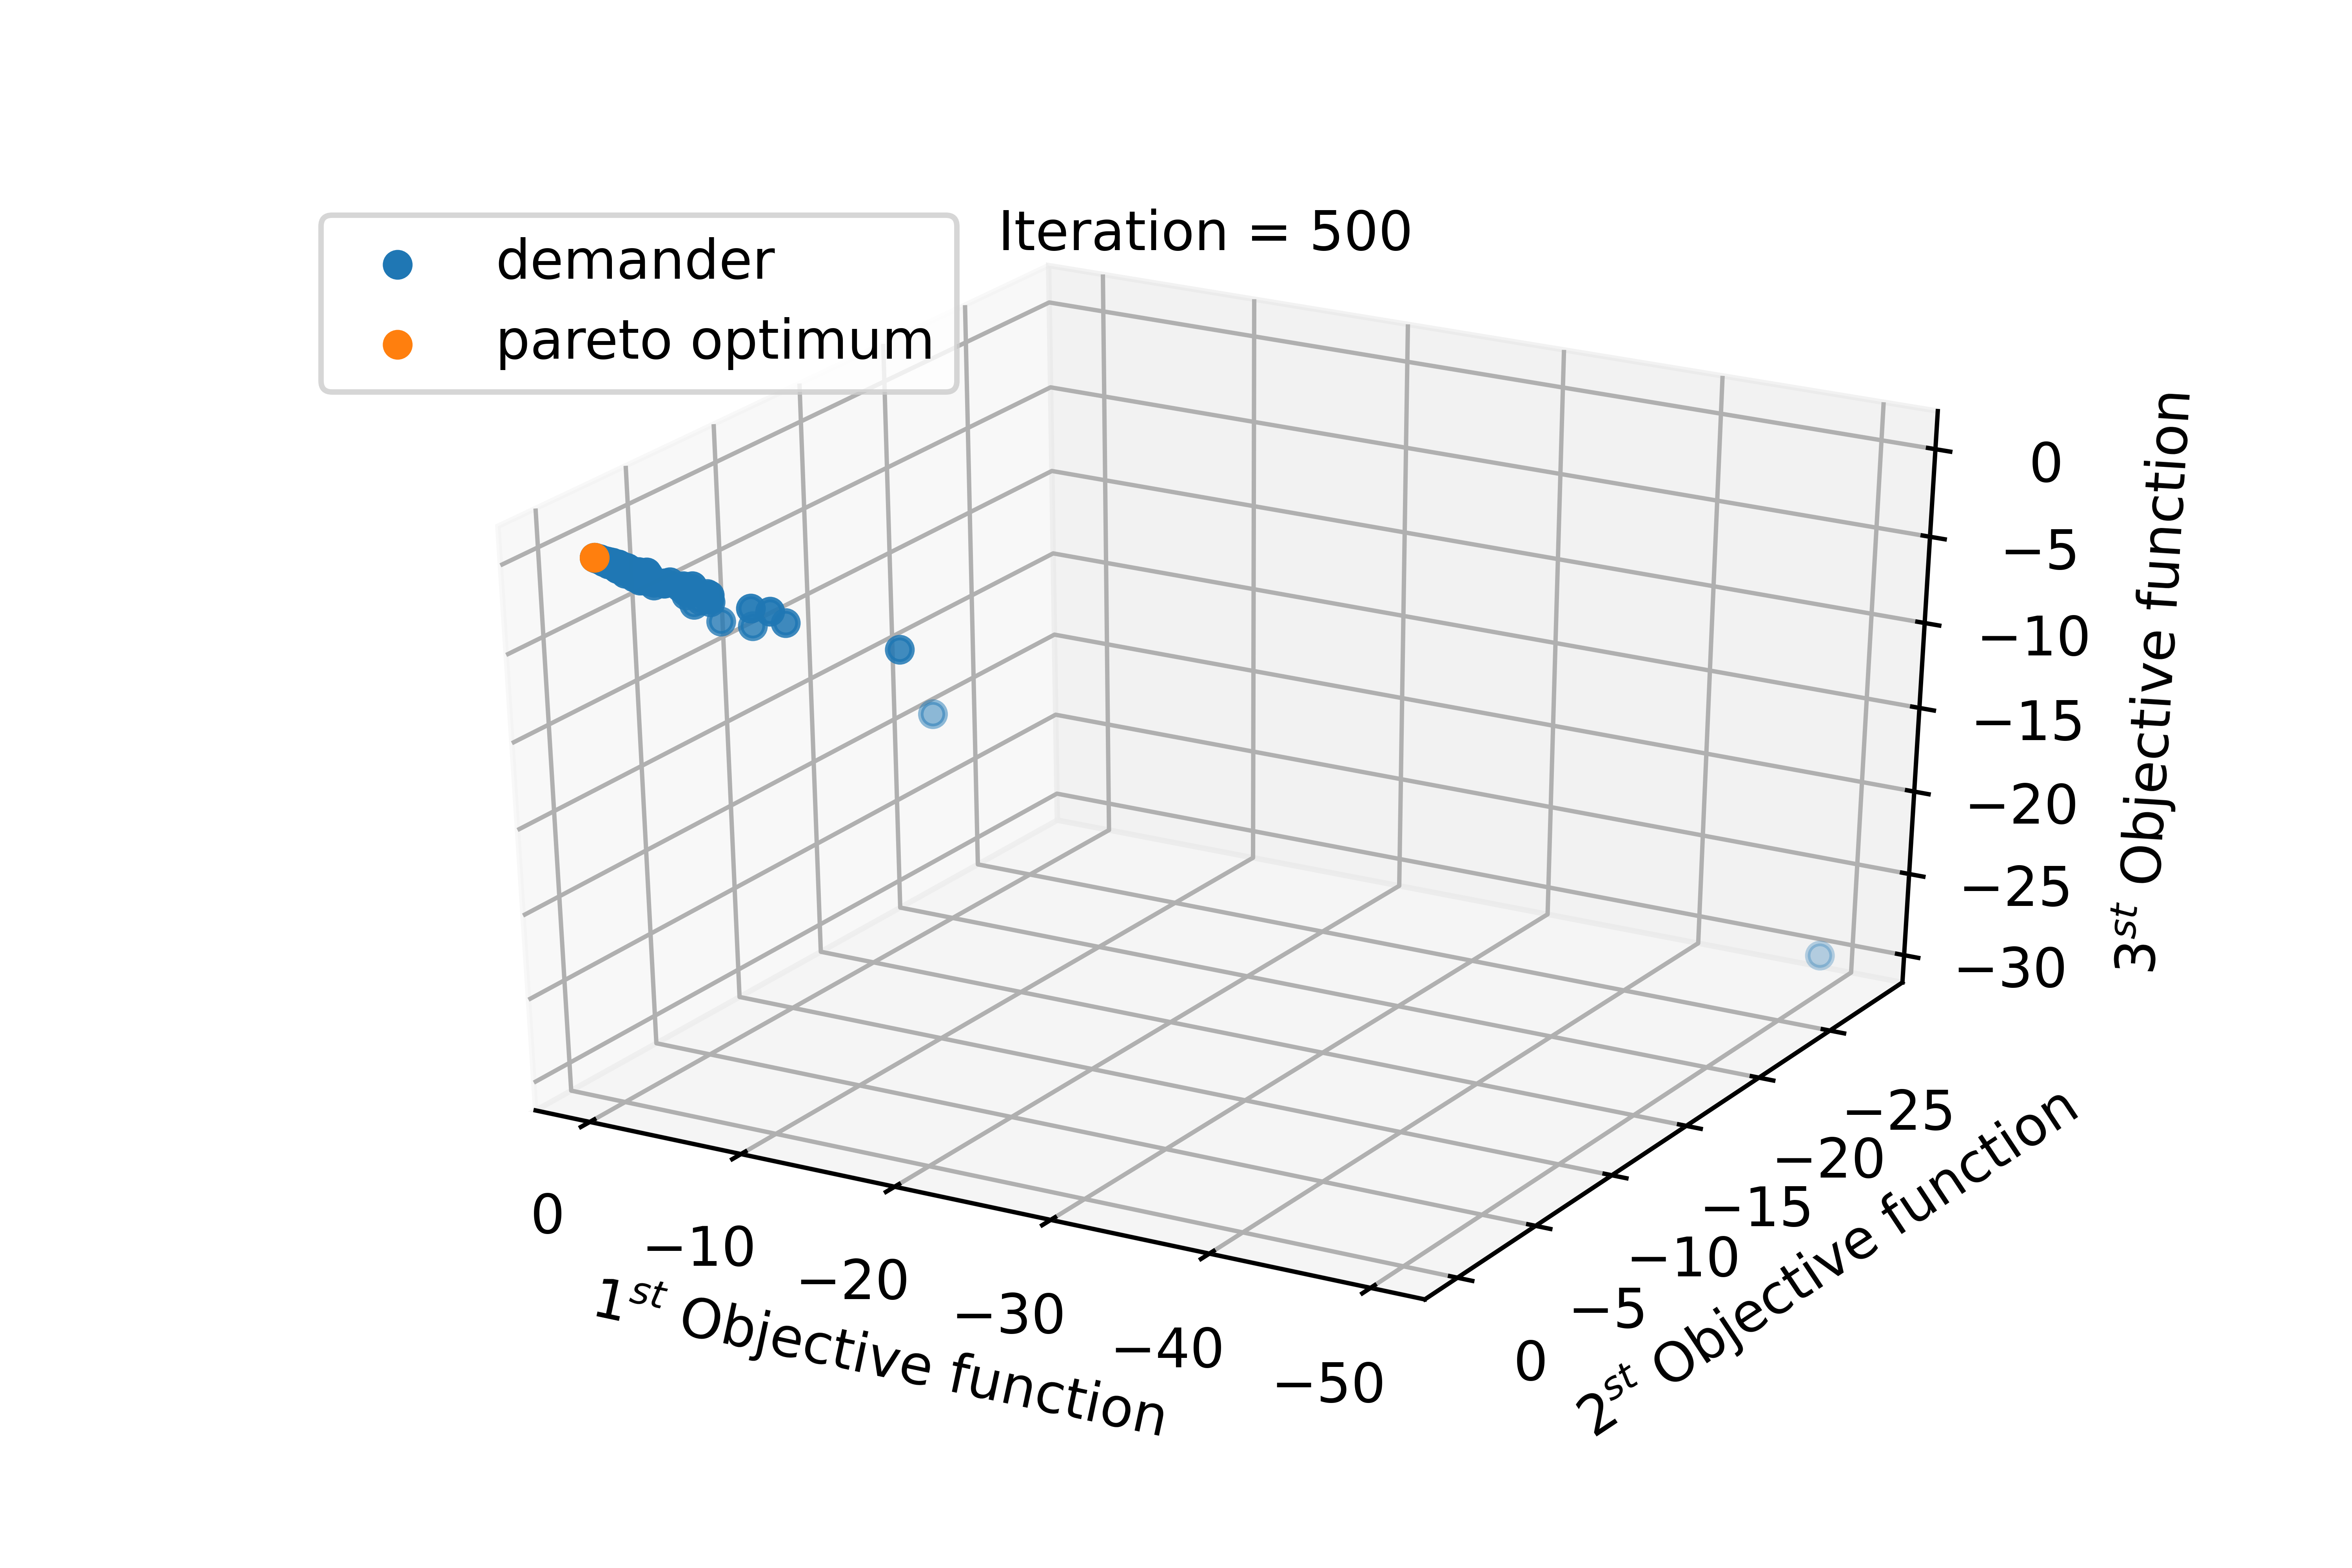
\includegraphics[width=1\linewidth]{../Figure/results/cooperative_3d_3.png}}
	\caption{مکان تقاضا‌کنندگان و بهینه پارتو در بهینه‌سازی چند هدفه هم جهت سه بعدی}
\end{figure}





\begin{table}[H]
	\caption{پارامترهای بهینه‌سازی چند هدفه هم جهت سه بعدی}
	\centering
	\begin{tabular}{|c|c|c|}
		\hline
		مقدار & پارامتر\\
		\hline
		$200$ 
		& تعداد تقاضا‌کنندگان\\
		$5$ 
		& نسبت تقاضاکنندگان به عرضه‌کنندگان \\
		$	10 $
		& نسبت تقاضاکنندگان به تعداد گروه دوستان\\
		$20$ 
		& نسبت زمان ساخت به زمان هر تکرار \\
		$0.7 $ &$K_{\sigma_D}$ \\
		$0.7$ &$K_{\sigma_S}$ \\
		$0.4$ &$K_{n_S}$ \\
		
		\hline
	\end{tabular}
\end{table}



\subsection{پیاده‌سازی توابع غیر هم جهت}

\begin{equation}
	\boldsymbol{f} = 
	\begin{cases}
		\sum_{i=0}^{D}(z_j-5)^2 \\
		\left(\sum_{i=1}^{D}\left(\sum_{j=1}^{i}z_j\right)^2\right)
	\end{cases}
\end{equation}



\begin{figure}[H]
	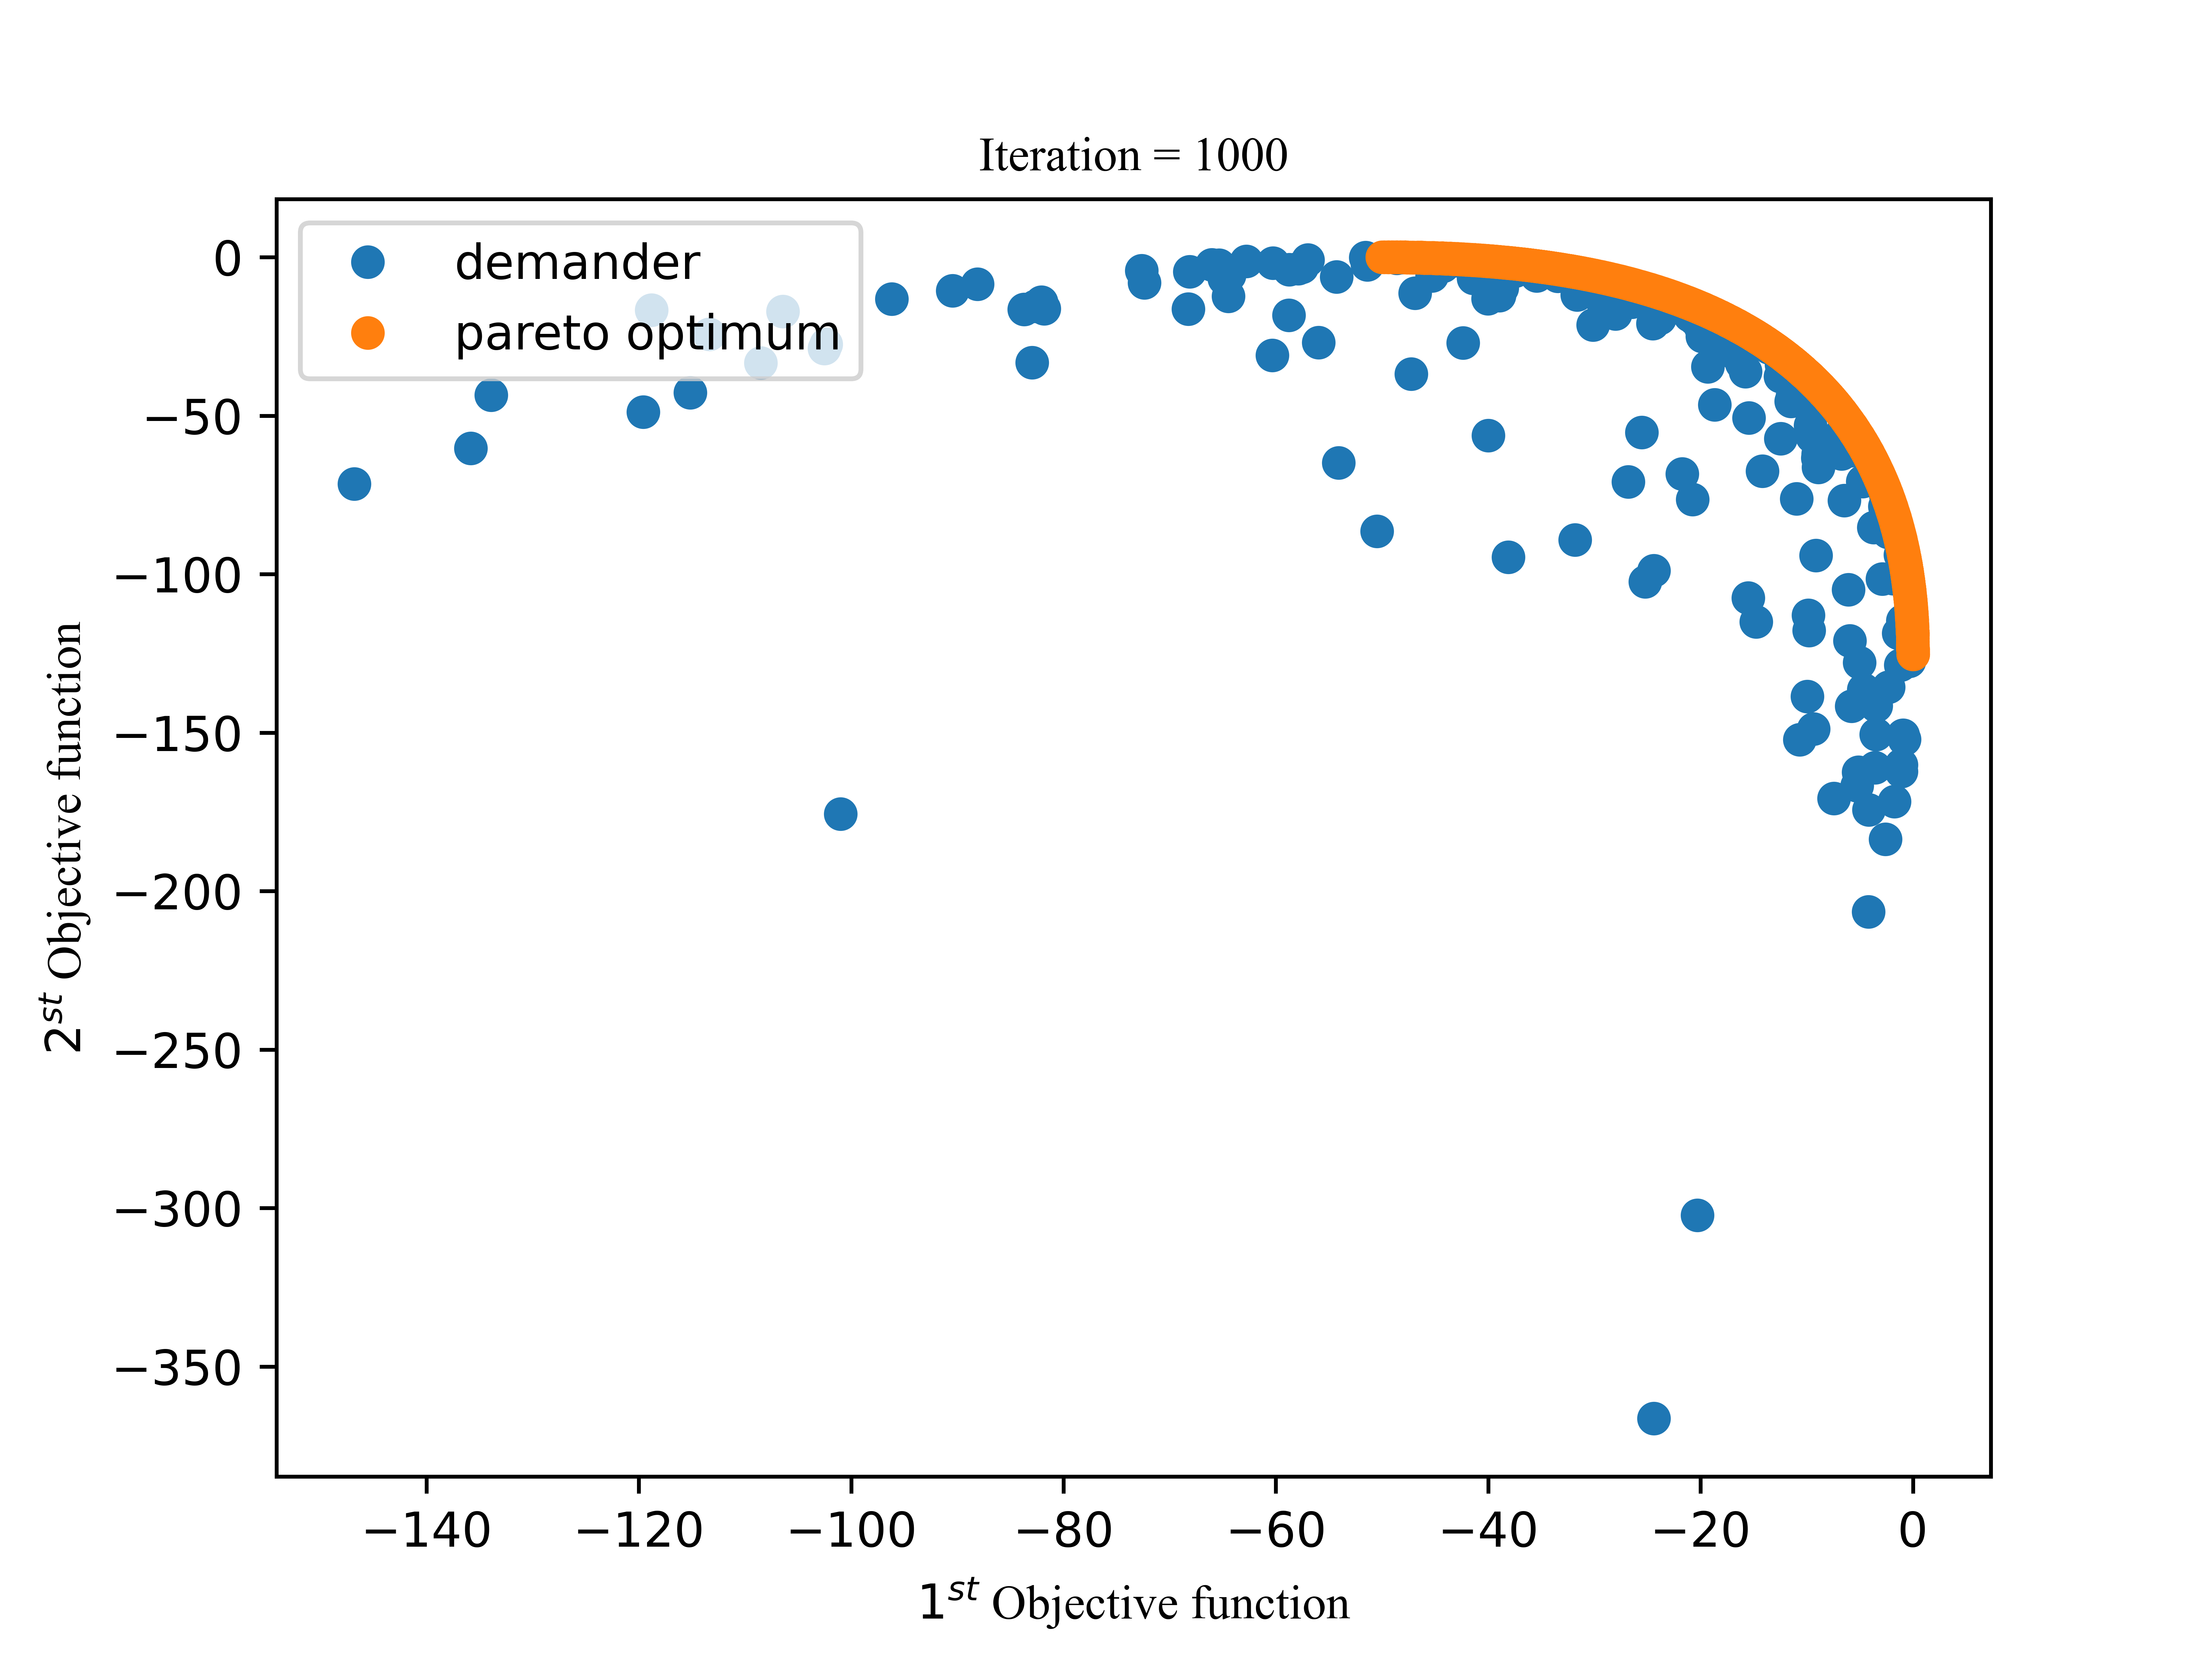
\includegraphics[width=16cm]{../Figure/results/non_cooperative_2d.png}
	\centering
	\caption{مکان تقاضا‌کنندگان و بهینه پارتو در بهینه‌سازی چند هدفه غیر هم جهت دو بعدی}
\end{figure}

\begin{table}[H]
	\caption{پارامترهای بهینه‌سازی چند هدفه غیر هم جهت دو بعدی}
	\centering
	\begin{tabular}{|c|c|c|}
		\hline
		مقدار & پارامتر\\
		\hline
		$200$ 
		& تعداد تقاضا‌کنندگان\\
		$5$ 
		& نسبت تقاضاکنندگان به عرضه‌کنندگان \\
		$	10 $
		& نسبت تقاضاکنندگان به تعداد گروه دوستان\\
		$20$ 
		& نسبت زمان ساخت به زمان هر تکرار \\
		$0.7 $ &$K_{\sigma_D}$ \\
		$0.7$ &$K_{\sigma_S}$ \\
		$0.4$ &$K_{n_S}$ \\
		
		\hline
	\end{tabular}
\end{table}









\begin{equation}
	\boldsymbol{f} = 
	\begin{cases}
		\sum_{i=0}^{D}(z_j-5)^2 \\
		\left(\sum_{i=1}^{D}\left(\sum_{j=1}^{i}z_j\right)^2\right) \\
		\left(\sum_{i=1}^{D}\left(\sum_{j=1}^{i}(z_j+5)\right)^2\right)(1+0.4\left\|N(0, 1))\right\|) 
	\end{cases}
\end{equation}


\begin{figure}[H]
	\centering
	\subfloat[]{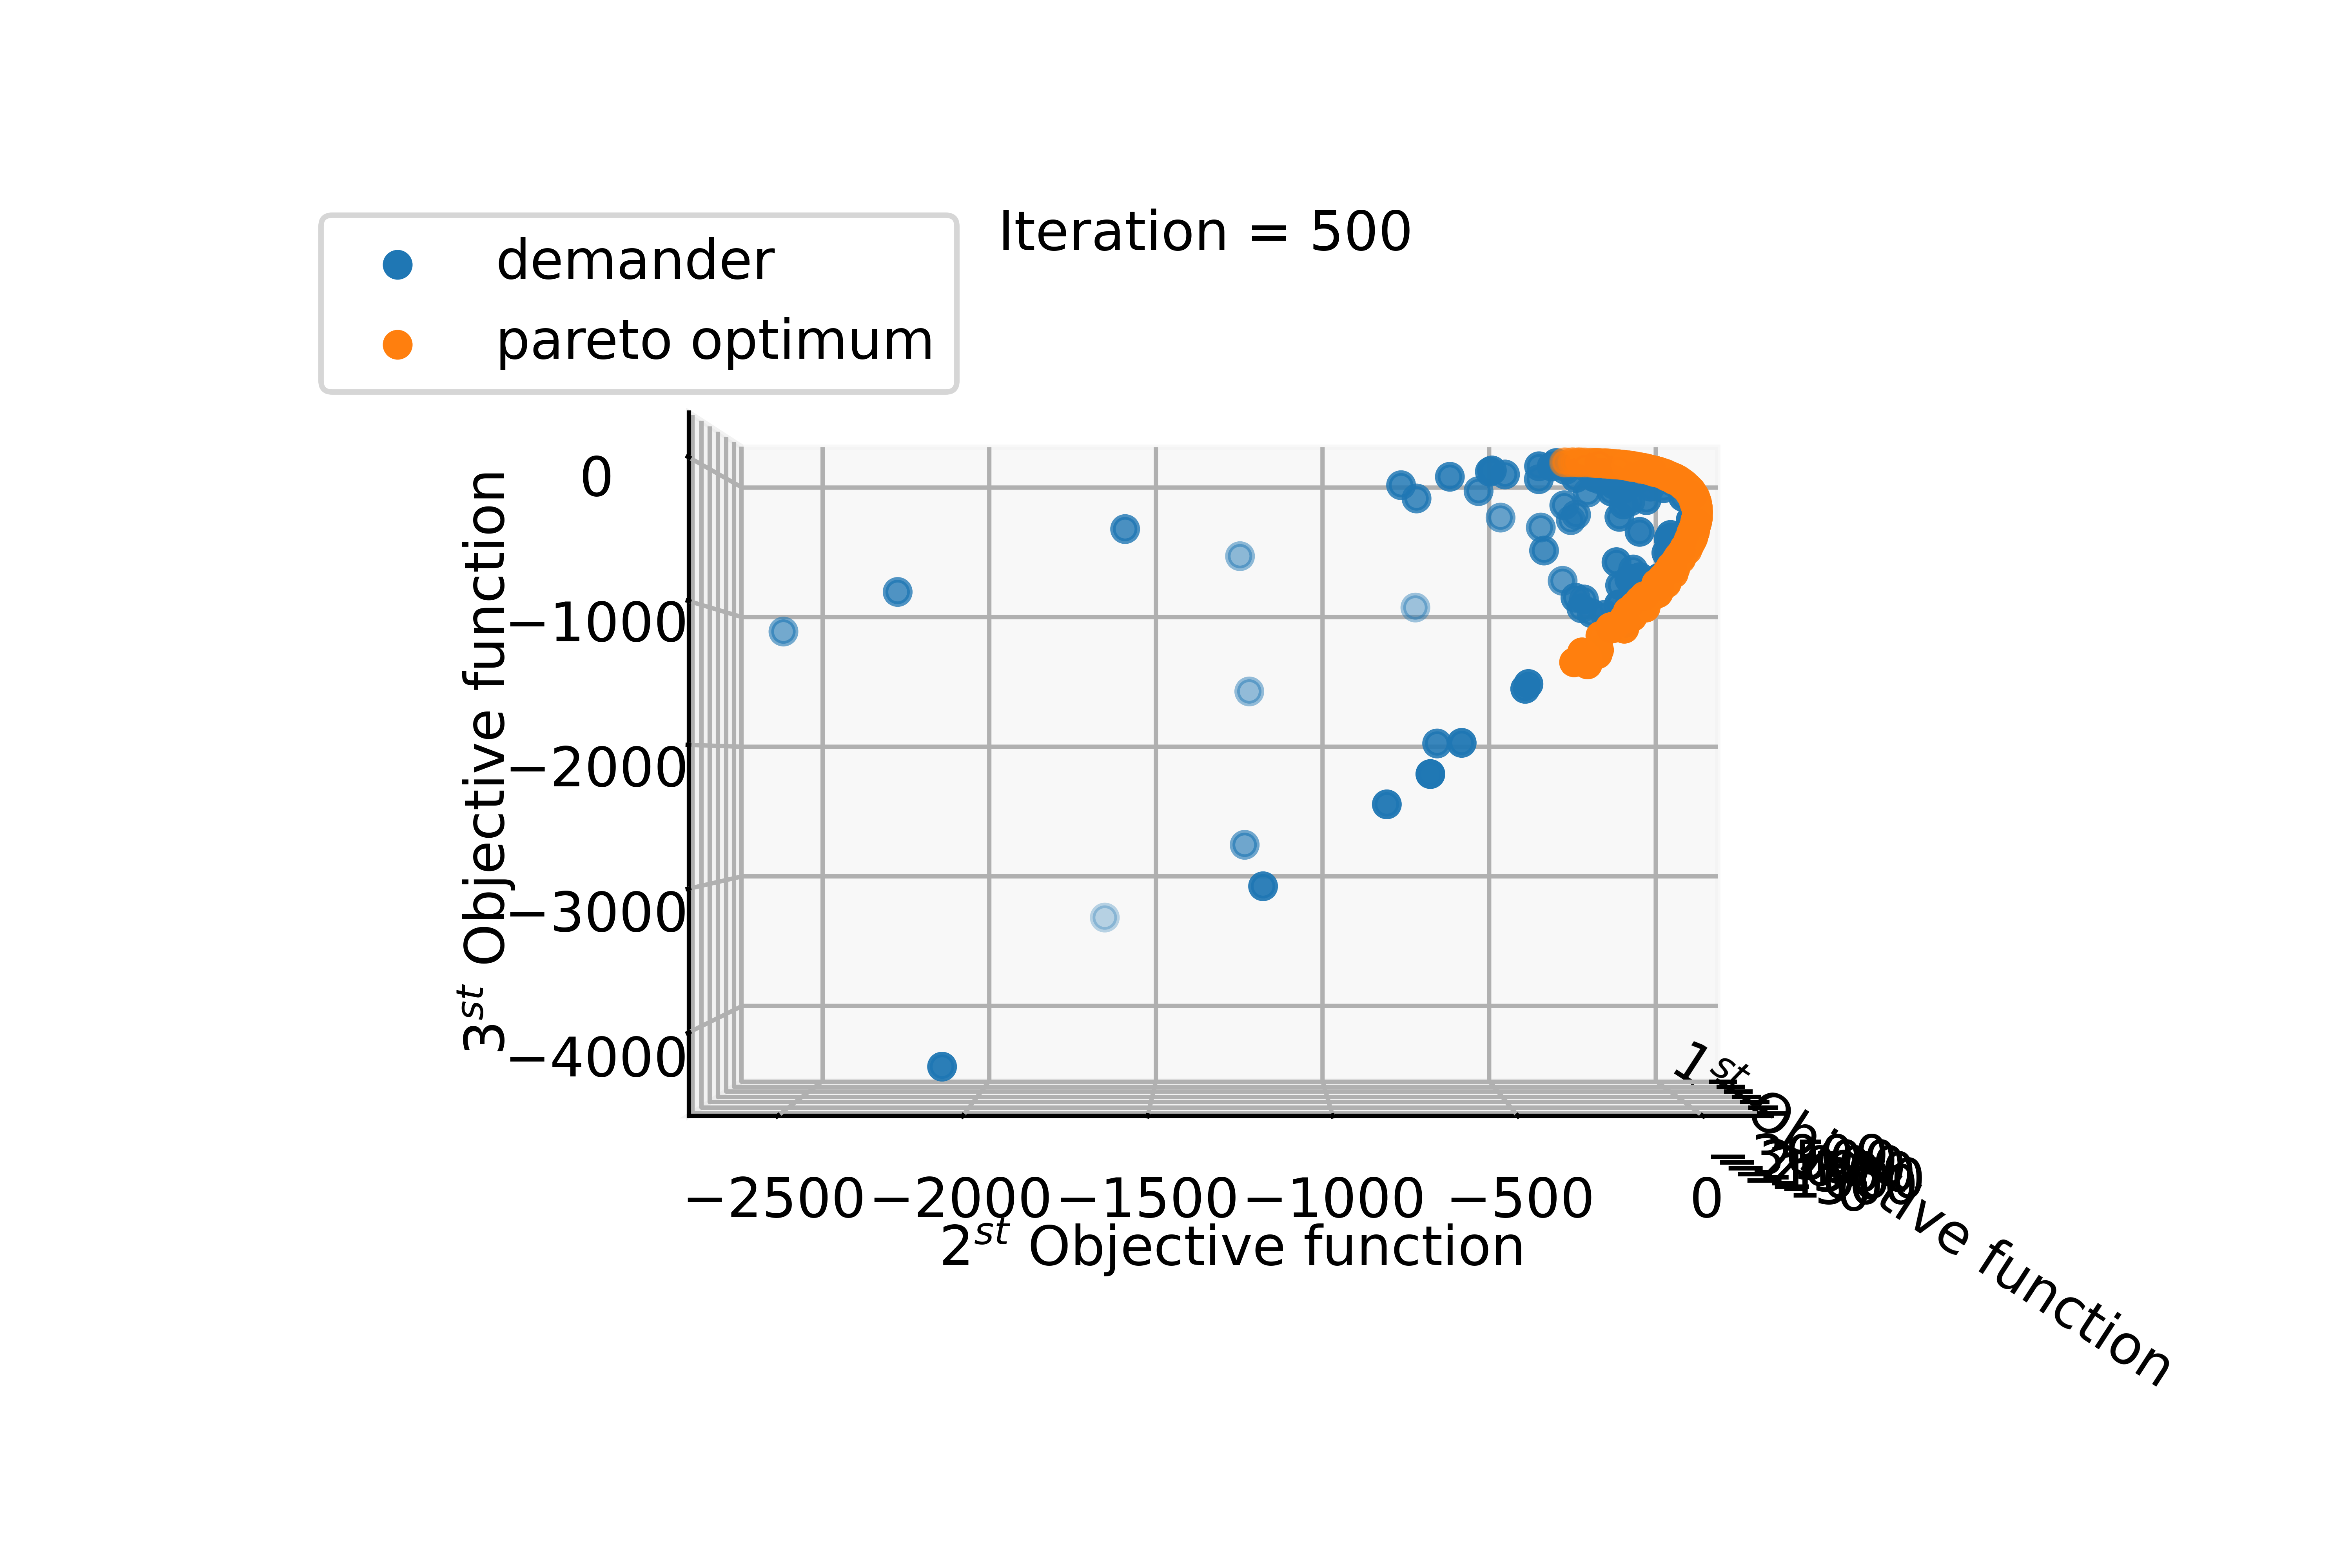
\includegraphics[width=.5\linewidth]{../Figure/results/non_cooperative_3d_1.png}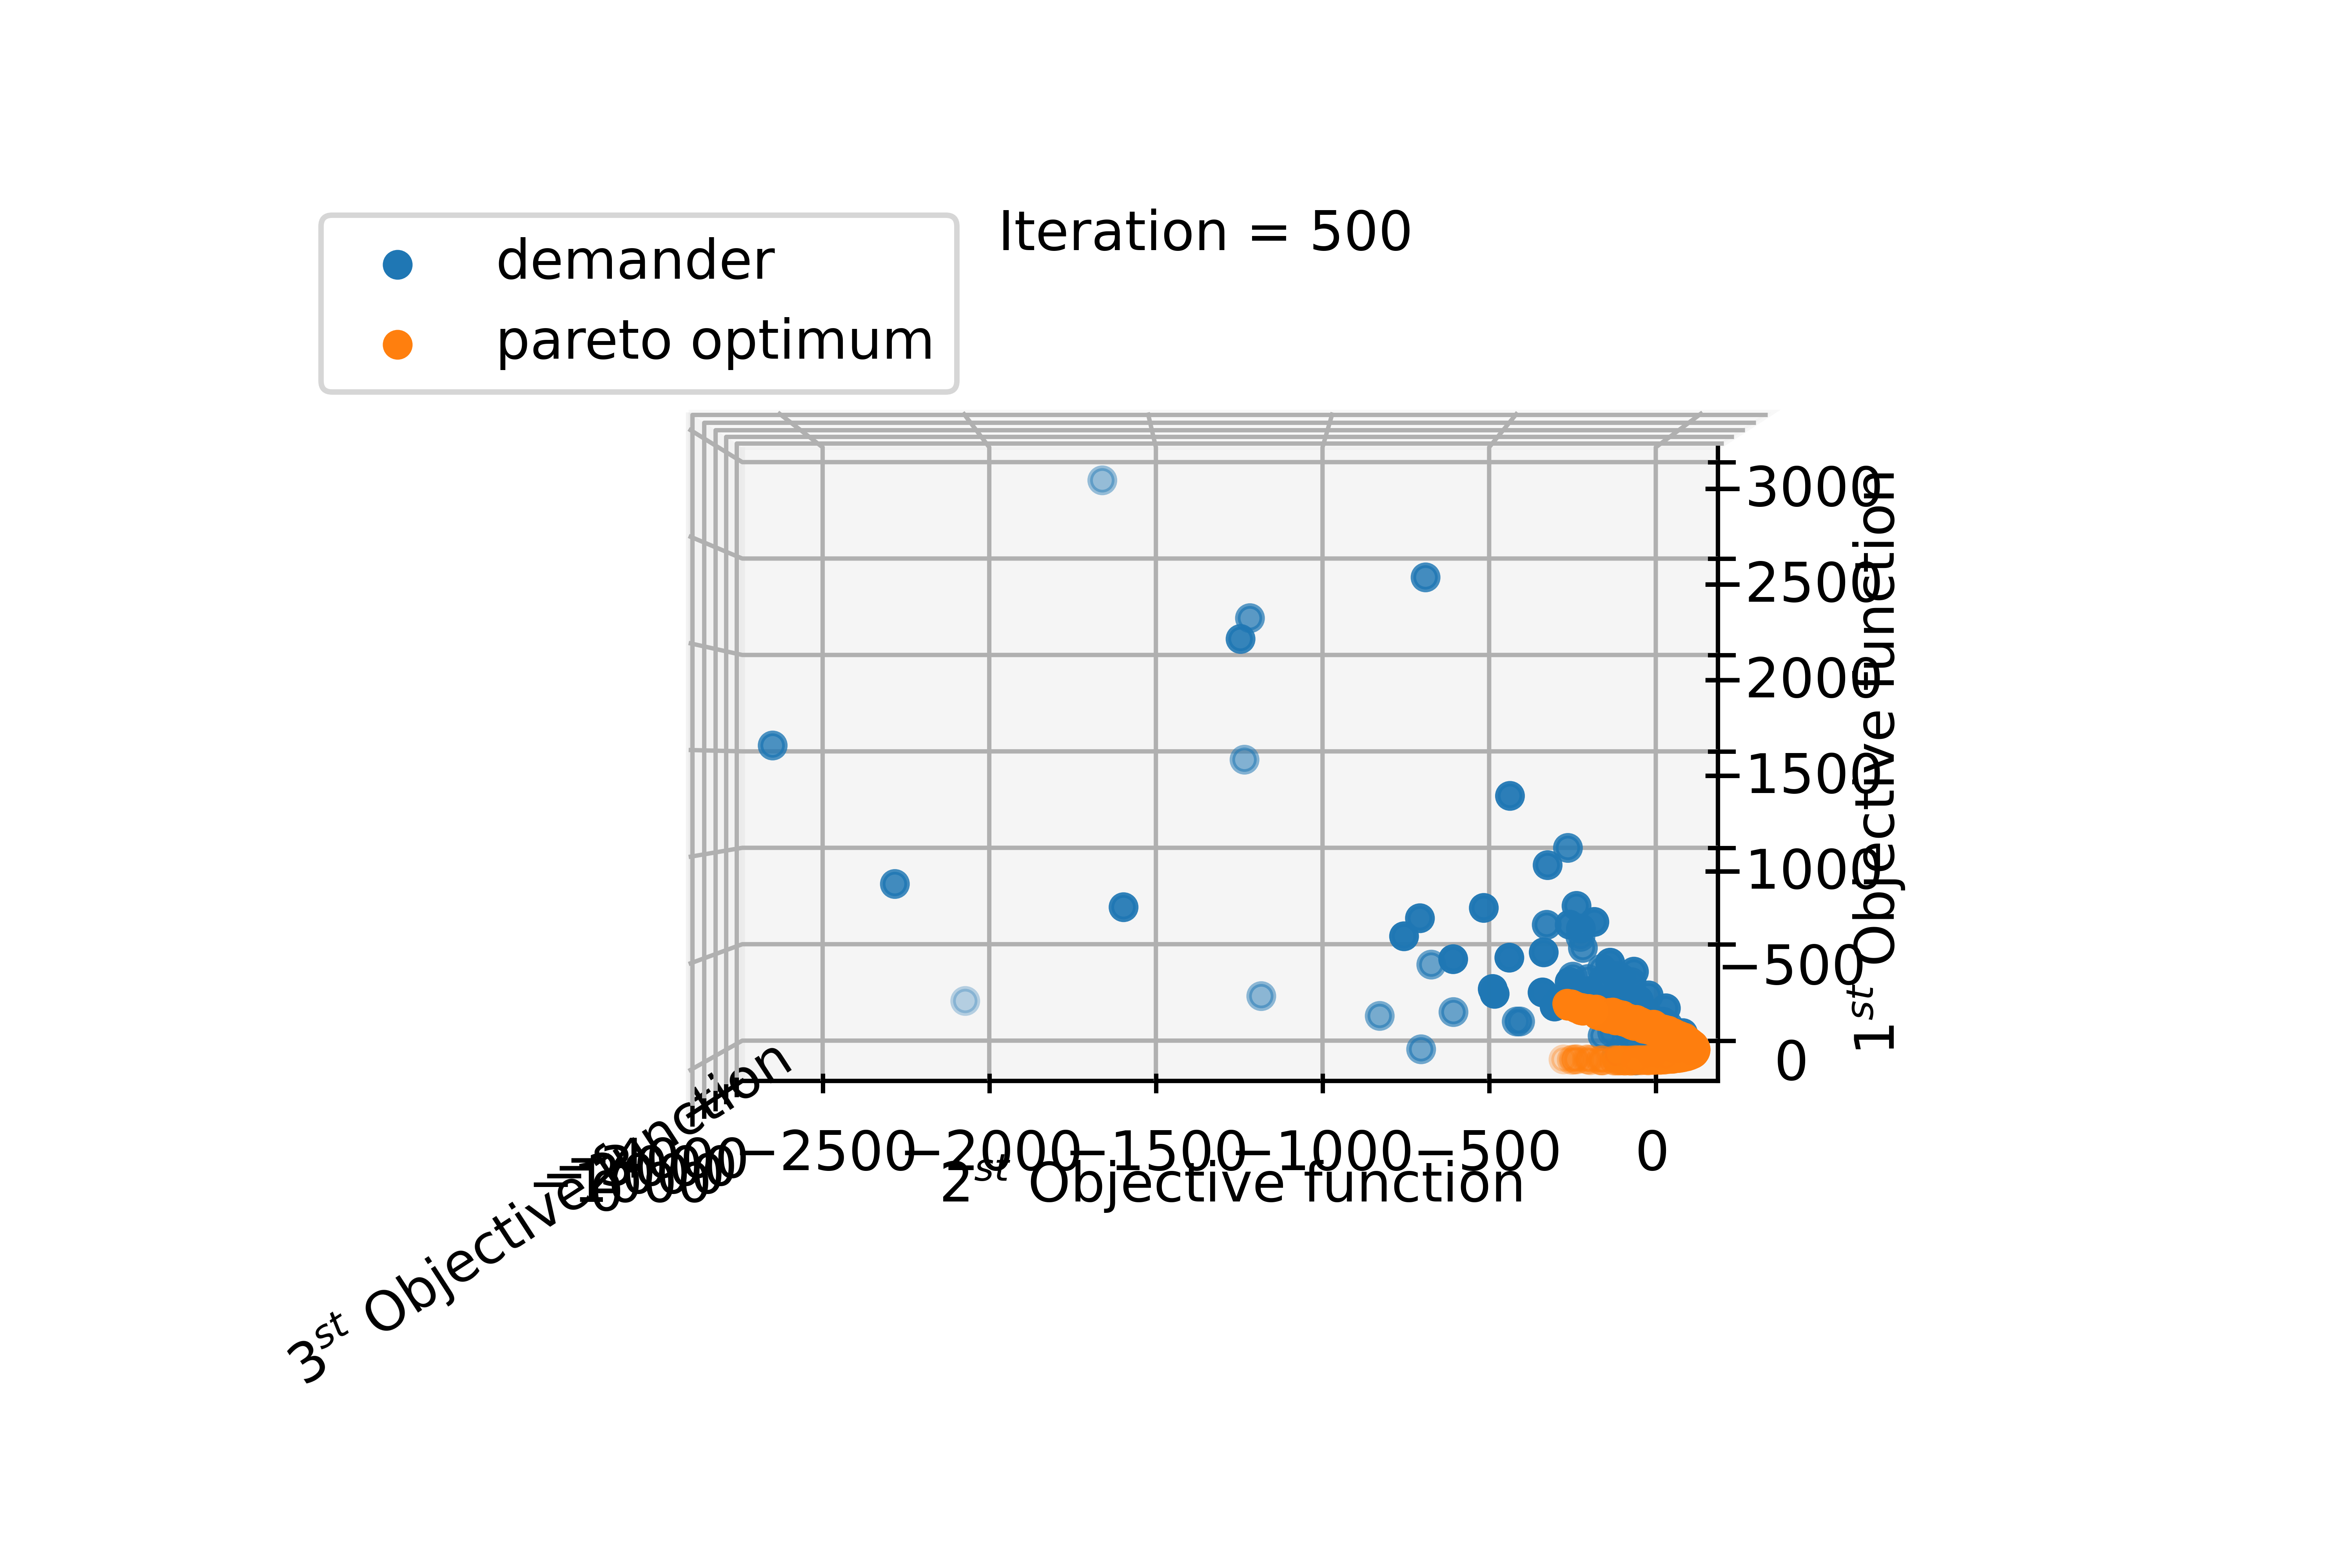
\includegraphics[width=.5\linewidth]{../Figure/results/non_cooperative_3d_2.png}}
	\hfill
	\subfloat[]{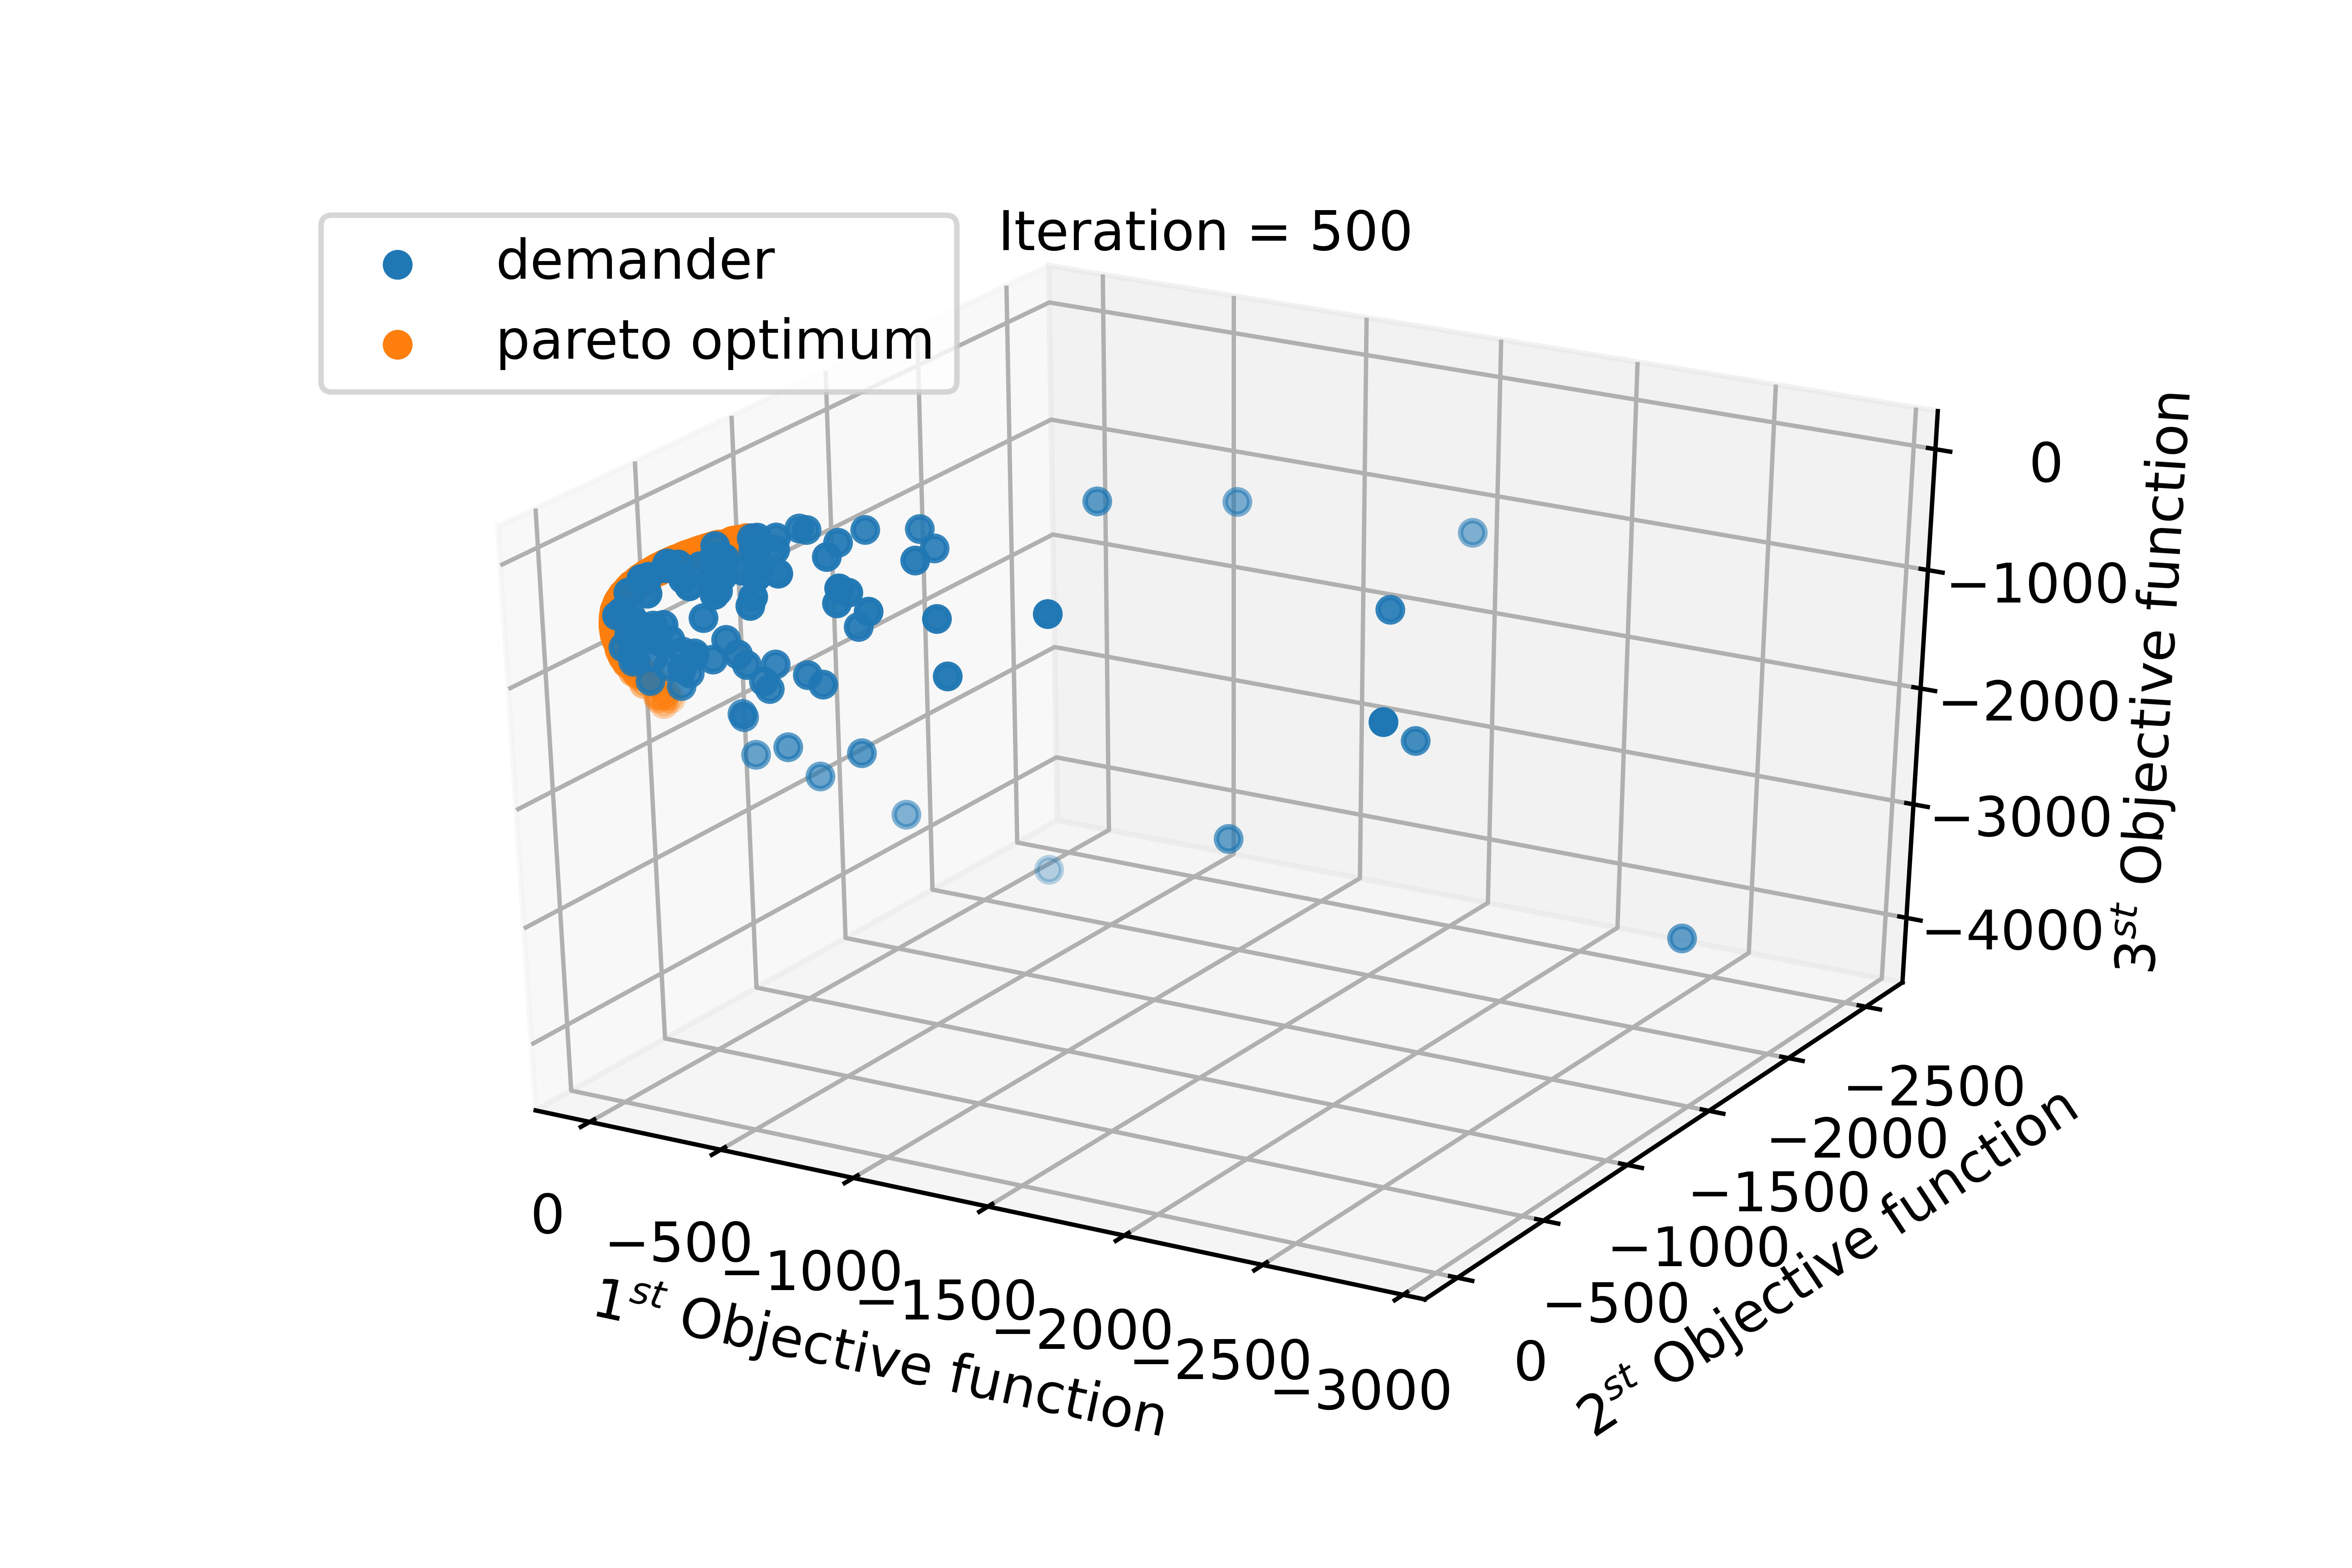
\includegraphics[width=1\linewidth]{../Figure/results/non_cooperative_3d_3.png}}
	\caption{مکان تقاضا‌کنندگان و بهینه پارتو در بهینه‌سازی چند هدفه غیر هم جهت سه بعدی}
\end{figure}

\begin{table}[H]
	\caption{پارامترهای بهینه‌سازی چند هدفه غیر هم جهت سه بعدی}
	\centering
	\begin{tabular}{|c|c|c|}
		\hline
		مقدار & پارامتر\\
		\hline
		$200$ 
		& تعداد تقاضا‌کنندگان\\
		$5$ 
		& نسبت تقاضاکنندگان به عرضه‌کنندگان \\
		$	10 $
		& نسبت تقاضاکنندگان به تعداد گروه دوستان\\
		$20$ 
		& نسبت زمان ساخت به زمان هر تکرار \\
		$0.7 $ &$K_{\sigma_D}$ \\
		$0.7$ &$K_{\sigma_S}$ \\
		$0.4$ &$K_{n_S}$ \\
		
		\hline
	\end{tabular}
\end{table}
 
 
 
 
 
 
 
 